\documentclass[sigconf, balance=false]{acmart}

\setcopyright{acmlicensed}
\copyrightyear{2026}
\acmYear{2026}
\acmDOI{XXXXXXX.XXXXXXX}

\acmConference[ACM Conf '26]{Make sure to enter the correct conference title from your rights confirmation email}{2026}{Location, Country}
\acmISBN{978-1-4503-XXXX-X/2026/XX}

\AtBeginDocument{%
  \providecommand\BibTeX{{%
    Bib\TeX}}}

\usepackage{tikz}
\usetikzlibrary{shapes.geometric, arrows.meta, positioning, fit, backgrounds, calc}
\usepackage{booktabs}
\usepackage{tabularx}
\usepackage{array}
\usepackage{multirow}
\usepackage{stfloats}
\usepackage{placeins}
\usepackage{enumitem}
\usepackage{xurl}

% Relax line-breaking penalties in narrow two-column layout to prevent margin overflows
\emergencystretch=1.5em
\sloppy

% Tune float placement parameters so figures and tables stay close to their text
\renewcommand{\topfraction}{0.95}
\renewcommand{\bottomfraction}{0.95}
\renewcommand{\textfraction}{0.05}
\renewcommand{\floatpagefraction}{0.85}
\renewcommand{\dbltopfraction}{0.95}
\renewcommand{\dblfloatpagefraction}{0.85}
\setcounter{topnumber}{5}
\setcounter{bottomnumber}{5}
\setcounter{totalnumber}{10}
\setcounter{dbltopnumber}{5}

\begin{document}

\title[The PANOPTES Reference Architecture]{PANOPTES: A Reference Architecture and Multimodal Correlation Engine for Cloud-Native Observability}

\author{Fagner Silva}
\authornote{Both authors contributed equally to this research.}
\affiliation{%
  \institution{Centro de Informática, UFPE}
  \city{Recife}
  \state{Pernambuco}
  \country{Brazil}
}
\email{ffcs@cin.ufpe.br}
\orcid{0000-0000-0000-0000}

\author{Jackson Raniel}
\affiliation{%
  \institution{Universidade de Pernambuco - Campus Caruaru}
  \city{Caruaru}
  \state{Pernambuco}
  \country{Brazil}
}
\email{jackson.florencio@upe.br}

\author{Vinícius Cardoso Garcia}
\authornotemark[1]
\affiliation{%
  \institution{Centro de Informática, UFPE}
  \city{Recife}
  \state{Pernambuco}
  \country{Brazil}
}
\email{vcg@cin.ufpe.br}

\renewcommand{\shortauthors}{Silva et al.}

\begin{abstract}
In cloud-native computing, microservices orchestrated by Kubernetes emit an overwhelming volume of heterogeneous telemetry across the three classical pillars: time-series metrics, structured logs, and distributed traces. However, existing industrial toolchains manage these modalities in fragmented silos, forcing Site Reliability Engineers (SREs) to perform manual dashboard correlation during critical outages. Furthermore, naive automated root-cause analysis (RCA) techniques that rely on a single modality suffer from acute architectural pathologies: inclusive span duration ranking suffers from a \textit{Cascading Span Bias} that consistently misattributes root causes to upstream API gateways ($0.00\%$ accuracy in our baselines), while native infrastructure monitoring remains completely blind to non-fatal resource saturation and network delays. Grounded in the epistemology of Design Science Research (DSR), this paper introduces \textbf{PANOPTES}, a novel 4-layer reference architecture and causal correlation engine for cloud-native observability. PANOPTES unifies non-invasive eBPF and OpenTelemetry probes (Layer 1), federated multimodal storage backends via OpenMetrics Exemplars (Layer 2), an algorithmic correlation engine utilizing exclusive Span Self-Time decomposition ($T_{\text{self}} = T_{\text{span}} - \sum T_{\text{child}}$) and cross-modal evidence fusion (Layer 3), and closed-loop diagnostic remediation (Layer 4). We instantiate PANOPTES on a Kubernetes testbed and evaluate it through a controlled, paired, stratified factorial experiment ($N=30$ campaigns) over the polyglot CNCF OpenTelemetry Astronomy Shop benchmark under Chaos Mesh fault injections. Our empirical findings demonstrate that PANOPTES achieves $\mathbf{83.33\%}$ ($25/30$) root-cause diagnostic accuracy, decisively outperforming monomodal distributed tracing ($0.00\%$, Fisher's exact $p = 5.49 \times 10^{-12}$) and native CLI inspection ($20.00\%$, $p = 1.55 \times 10^{-6}$). Furthermore, PANOPTES slashes median diagnostic latency ($MTTDiag$) by $\mathbf{94.24\%}$ (from $300.00\,\text{s}$ to $\mathbf{17.27\,\text{s}}$, Wilcoxon $p = 1.35 \times 10^{-4}$, Vargha-Delaney $\hat{A}_{12} = 0.817$), while strictly bounding the dedicated observability CPU overhead to $\mathbf{5.26\% \pm 2.65\%}$ of the monitored workload ($131.17 \pm 66.26\,\text{mCPU}$), proving that comprehensive multimodal correlation can be achieved without compromising cluster stability.
\end{abstract}

\begin{CCSXML}
<ccs2012>
   <concept>
       <concept_id>10011007.10011074.10011075</concept_id>
       <concept_desc>Software and its engineering~Software architectures</concept_desc>
       <concept_significance>500</concept_significance>
   </concept>
   <concept>
       <concept_id>10011007.10011074.10011099.10011102.10011103</concept_id>
       <concept_desc>Software and its engineering~Software testing and debugging</concept_desc>
       <concept_significance>500</concept_significance>
   </concept>
   <concept>
       <concept_id>10010520.10010521.10010537.10003100</concept_id>
       <concept_desc>Computer systems organization~Cloud computing</concept_desc>
       <concept_significance>500</concept_significance>
   </concept>
 </ccs2012>
\end{CCSXML}

\ccsdesc[500]{Software and its engineering~Software architectures}
\ccsdesc[500]{Software and its engineering~Software testing and debugging}
\ccsdesc[500]{Computer systems organization~Cloud computing}

\keywords{Cloud-Native, Observability, Reference Architecture, Multimodal Correlation, Microservices, Design Science Research, Root Cause Analysis, Kubernetes}

\maketitle

\section{Introduction}
\label{sec:introduction}

The widespread adoption of cloud-native computing and container orchestration platforms, led by Kubernetes, has transformed contemporary software systems into complex distributed webs of loosely coupled microservices \cite{gannon_2017, bogner2020microservices}. While this architectural paradigm accelerates feature delivery, independent scalability, and organizational agility, it fundamentally complicates operational visibility. When transient network anomalies, CPU saturation, or pod failures occur within polyglot service graphs, failure symptoms cascade across remote procedure calls (RPC) and event brokers, obfuscating the actual root cause \cite{soldani2022anomaly, zhou2021fault}.

To diagnose such failures, modern DevOps and Site Reliability Engineering (SRE) teams collect the ``Three Pillars of Observability'': numerical time-series metrics, structured event logs, and distributed trace spans \cite{sridharan_2018, beyer2016sre}. However, in current industrial practice and academic literature, these telemetry modalities are frequently managed in fragmented silos \cite{kosinska_2023, nedelkoski2020selfattentive}. SREs are forced to manually correlate dashboard anomalies in Prometheus with unstructured text logs in Grafana Loki and call trees in Grafana Tempo or Jaeger. This manual triaging prolongs the Mean Time to Diagnose ($MTTDiag$), heightens cognitive load, and frequently leads to erroneous incident remediation.

Furthermore, naive automated Root Cause Analysis (RCA) approaches that rely on a single telemetry modality suffer from severe architectural limitations:
\begin{itemize}[leftmargin=1.2em, itemsep=2pt, topsep=3pt]
    \item \textbf{Cascading Span Bias in Monomodal Tracing:} Naive trace diagnostic algorithms that isolate culprits by ranking inclusive span durations invariably point to upstream ingress microservices (e.g., API gateways or edge proxies), misidentifying victims of accumulated downstream latency as the source of failure \cite{yu2021microrank}.
    \item \textbf{Semantic Blindness in Monomodal Metrics:} System-level metric scrapers capture host resource spikes (e.g., CPU, RAM) but lack transaction context, making them incapable of distinguishing between legitimate user traffic surges and rogue background processes.
    \item \textbf{Invasiveness and Observability Tax:} Increasing probe frequency and capturing un-sampled traces across high-throughput clusters introduces non-negligible CPU and memory overhead, perturbing application performance and risking the very stability observability seeks to ensure \cite{vancamp24, valbusa_2025}.
\end{itemize}

Despite these pressing dilemmas, the software engineering community lacks a formal, empirically validated reference architecture that defines how multimodal telemetry streams should be semantically unified, correlated, and bounded in resource footprint. 

To bridge this gap, this paper introduces \textbf{PANOPTES}, a novel reference architecture and multimodal correlation engine for cloud-native microservice observability. Grounded in the epistemology of \textbf{Design Science Research (DSR)} \cite{simon_1969, hevner_2004, peffers_2007}, PANOPTES delivers a 4-layer reference model that unifies non-invasive eBPF and OpenTelemetry probes, federated multimodal storage backends, and a causal correlation engine powered by intra-trace \textit{Span Self-Time Decomposition} ($T_{\text{self}}$) and OpenMetrics Exemplar binding.

Specifically, this research addresses three core Research Questions (RQs):
\begin{itemize}[leftmargin=1.2em, itemsep=2pt, topsep=3pt]
    \item \textbf{RQ1 (Architectural Design \& Semantic Invariants):} What structural layers, semantic bindings, and design heuristics are necessary to eliminate telemetry silos and prevent Cascading Span Bias in distributed microservices?
    \item \textbf{RQ2 (Diagnostic Efficacy \& Latency Reduction):} How effectively does the PANOPTES multimodal correlation engine isolate root causes under cascading chaos perturbations compared to native Kubernetes inspection and monomodal distributed tracing?
    \item \textbf{RQ3 (Resource Overhead \& Invasiveness Envelope):} What is the steady-state CPU and memory footprint imposed by the complete PANOPTES reference stack, and can it be bounded within a predictable operational envelope?
\end{itemize}

Through a rigorous controlled experiment over the polyglot CNCF OpenTelemetry Astronomy Shop benchmark ($N=30$ paired trials, stratified across network delay, pod termination, and CPU stress), we demonstrate that PANOPTES achieves $\mathbf{83.33\%}$ diagnostic accuracy, outperforming monomodal tracing ($0.00\%$, $p < 10^{-11}$) and native CLI inspection ($20.00\%$, $p < 10^{-6}$), while reducing median $MTTDiag$ from $300.00\,\text{s}$ to $\mathbf{17.27\,\text{s}}$ and bounding observability CPU overhead to under $10\%$ of cluster capacity.

\section{Background and Problem Grounding}
\label{sec:background}

\subsection{Cloud-Native Telemetry Modalities: Metrics, Logs, and Traces}
In distributed architectures orchestrated by Kubernetes, observability relies on three complementary data modalities:
\begin{enumerate}[leftmargin=1.2em, itemsep=2pt, topsep=3pt]
    \item \textbf{Numerical Metrics ($\mathcal{M}$):} Numeric, timestamped aggregations of operational indicators (e.g., container CPU millicores, cgroup memory working sets, network socket drop rates). Metrics are computationally efficient to scrape, store, and query via domain-specific engines like Prometheus (TSDB) using PromQL. However, metrics lack individual transaction context and request-level execution causality.
    \item \textbf{Structured Logs ($\mathcal{L}$):} Semi-structured, discrete text events generated by application runtimes and container engines (e.g., standard output, stack traces, \texttt{SIGTERM} shutdown notices). Modern log aggregators such as Grafana Loki index streams by metadata labels (namespace, pod name) rather than full-text indexing, optimizing storage footprint while allowing regex-based log streaming via LogQL.
    \item \textbf{Distributed Traces ($\mathcal{T}$):} Directed Acyclic Graphs (DAGs) representing end-to-end execution paths of distributed requests traversing multi-tier microservices \cite{sigelman_2010}. Propagated across network hops via standardized metadata headers (e.g., W3C TraceContext), traces consist of individual spans denoting timed units of work with parent-child relationships.
\end{enumerate}

\subsection{The Diagnostic Dilemma in Unimodal Observability}
Although modern microservices instrument all three pillars, existing root-cause analysis (RCA) techniques typically process them in isolation, triggering three fundamental pathologies:

\subsubsection{The Cascading Span Bias in Distributed Tracing}
Consider an upstream edge gateway ($S_{\text{edge}}$) invoking a chain of internal services $S_1 \rightarrow S_2 \rightarrow S_3$, where $S_3$ experiences a severe network partition or $2000\,\text{ms}$ socket timeout. Because parent spans synchronously enclose the latency of all downstream child spans:
\begin{equation}
\begin{split}
    T_{\text{inclusive}}(S_{\text{edge}}) &> T_{\text{inclusive}}(S_1) \\
    &> T_{\text{inclusive}}(S_2) \ge T_{\text{inclusive}}(S_3)
\end{split}
\end{equation}
Any naive diagnostic algorithm that evaluates span degradation solely by absolute span duration will flag $S_{\text{edge}}$ as the slowest service in the trace. We formally designate this pathology as the \textbf{Cascading Span Bias}. In our baseline experiments, this bias induces a catastrophic $0.00\%$ root-cause accuracy, as the edge gateway is consistently and erroneously indicted for downstream faults.

\subsubsection{The Silent Metric Trap in Infrastructure Monitoring}
Infrastructure metrics are scraped asynchronously at coarse intervals (typically $15\,\text{s}$ to $60\,\text{s}$ to mitigate scraper overhead). When a container experiences a short-lived micro-burst or non-fatal thread contention, the aggregated metric averages out the perturbation. Conversely, when a container terminates abruptly due to a \texttt{SIGKILL} signal, metric scrapers simply lose the target, resulting in missing data rather than an explicit anomaly signal. Without correlated container crash logs, metrics alone cannot pinpoint the failure trigger.

\subsubsection{The Observability Tax and Invasiveness Envelope}
Injecting deep in-process instrumentation hooks across polyglot microservice runtimes (Java Virtual Machines, Node.js V8 engines, Python interpreters, Go binaries) introduces significant CPU and memory bloat, thread contention, and garbage collection pauses \cite{vancamp24, valbusa_2025}. An unconstrained observability pipeline can consume over $30\%$ of total node memory in resource-constrained edge or cloud deployments, transforming the monitoring infrastructure itself into a primary source of cluster instability.

\subsection{Guiding Control Principles for Multimodal Observability}
To overcome these limitations, we formulate two fundamental engineering control principles that govern the PANOPTES reference architecture:
\begin{itemize}[leftmargin=1.2em, itemsep=2pt, topsep=3pt]
    \item \textbf{Control Principle 1 (CP1 — Least Invasive Observation):} Telemetry collection must maximize diagnostic entropy reduction while strictly bounding the dedicated observability control-plane footprint within a predictable resource envelope ($\le 10\%$ CPU, $\le 20\%$ RAM of the monitored workload).
    \item \textbf{Control Principle 2 (CP2 — Semantic Continuity):} Causal context must be deterministically preserved across asynchronous IPC and protocol boundaries by decoupling parent-child inclusive latencies and binding discrete logs and metric time series directly to trace spans via OpenMetrics Exemplars.
\end{itemize}

\section{Design Science Research Methodology}
\label{sec:dsr_methodology}

Unlike traditional natural science methodologies that aim to discover and explain existing phenomena, Design Science Research (DSR) is rooted in pragmatic epistemology \cite{simon_1969}. DSR focuses on creating and evaluating innovative artifacts that solve identified operational problems, extending human and organizational capabilities while contributing prescriptive knowledge to the scientific body of knowledge \cite{hevner_2004, gregor_2013}.

In this research, we adopt the formal Design Science Research Methodology (DSRM) process model articulated by Peffers et al. \cite{peffers_2007}. As summarized in Table~\ref{tab:dsr_elements}, our research cycle operationalizes the six sequential DSRM activities:

\begin{table*}[!htbp]
\centering
\small
\caption{Design Science Research (DSR) Framework Mapping for the PANOPTES Reference Architecture}
\label{tab:dsr_elements}
\begin{tabularx}{\textwidth}{@{}l p{4.2cm} X@{}}
\toprule
\textbf{DSR Dimension} & \textbf{Epistemological Definition} & \textbf{Operationalization in PANOPTES} \\ \midrule
\textbf{Problem Domain} & Real-world operational dilemma in cloud-native microservices & Elevated Mean Time to Diagnose ($MTTDiag$), diagnostic inaccuracy under cascading faults, and unquantified probe overhead in distributed container environments (Wicked Problem). \\ \addlinespace[2pt]
\textbf{Class of Problems} & Generalized software engineering challenge & Automated, real-time correlation across heterogeneous, asynchronous telemetry modalities (metrics, logs, traces) without degrading host/cgroup performance. \\ \addlinespace[2pt]
\textbf{Artifact Type} & Prescriptive scientific contribution (Vaishnavi \& Kuechler) & \textbf{Model / Architecture:} Structural 4-layer reference framework with formal semantic bindings; \textbf{Method:} Span self-time ($T_{\text{self}}$) decomposition and exemplar correlation; \textbf{Instantiation:} Kubernetes IaC stack (Prometheus, Loki, Tempo, eBPF, OTel Collector). \\ \addlinespace[2pt]
\textbf{Design Principles} & Foundational engineering heuristics (Hevner et al., Walls et al.) & \textbf{Control Principles (\texttt{CP1}--\texttt{CP2}):} Non-invasive causal linkage ($\le 10\%$ CPU) and unified semantic representation (OTLP/Exemplars); \textbf{Contingency Heuristics (\texttt{ConH1}--\texttt{ConH3}):} Declarative control (IaC/CRDs), configuration drift rejection, and adaptive feedback to contain the Observer Effect. \\ \addlinespace[2pt]
\textbf{Evaluation Rigor} & Multi-criteria artifact evaluation (Hevner et al.) & Technical feasibility and overhead benchmarking (CP1 verification) coupled with architectural utility validation across $N=30$ stratified failure scenarios on CNCF Astronomy Shop. \\ \bottomrule
\end{tabularx}
\end{table*}


\begin{enumerate}[leftmargin=1.2em, itemsep=3pt, topsep=4pt]
    \item \textbf{Problem Identification and Motivation:} As characterized in Section~\ref{sec:background}, diagnosing distributed cloud-native failures is hindered by telemetry silos, the Cascading Span Bias, and uncontrolled probe overhead. These challenges constitute a ``wicked problem'' characterized by complex interdependencies and conflicting trade-offs between diagnostic accuracy and resource overhead.
    \item \textbf{Define Objectives of a Solution:} The objectives are quantitatively formalized through our three Research Questions (RQ1--RQ3): (i) establish an architecturally unified, 4-layer reference framework with formal semantic invariants; (ii) achieve $>80\%$ automated root-cause accuracy under multi-class chaos perturbations; and (iii) constrain total observability CPU overhead to $\le 10\%$ of cluster capacity.
    \item \textbf{Design and Development (The Artifact):} Following the artifact taxonomy of Vaishnavi and Kuechler \cite{vaishnavi_2015}, PANOPTES delivers three complementary contributions:
    \begin{itemize}[leftmargin=1.0em, itemsep=1pt]
        \item \textit{Model / Reference Architecture:} A 4-layer conceptual model establishing clean separation between ingestion, storage, correlation, and remediation.
        \item \textit{Method / Algorithms:} A deterministic causal correlation algorithm based on exclusive Span Self-Time decomposition ($T_{\text{self}}$) and multimodal evidence fusion.
        \item \textit{Instantiation:} A fully automated Kubernetes-native deployment pipeline codified in Ansible playbooks, Helm charts, and custom OpenTelemetry Collector pipelines.
    \end{itemize}
    \item \textbf{Demonstration:} We instantiate the PANOPTES reference architecture within an isolated, multi-node Kubernetes testbed running the CNCF OpenTelemetry Astronomy Shop benchmark, simulating real-world e-commerce microservice traffic under Locust user load.
    \item \textbf{Evaluation (Artifact Validation \& Benchmarking):} Following the evaluation taxonomy of Hevner et al. \cite{hevner_2004} and Gregor and Hevner \cite{gregor_2013}, we evaluate the artifact along three complementary dimensions: (i) \textit{Technical Feasibility and Invasiveness} by benchmarking the steady-state CPU and memory overhead against Control Principle \textbf{CP1}; (ii) \textit{Methodological Soundness and Diagnostic Utility} by comparing the PANOPTES correlation method ($T_{\text{self}}$ and multimodal evidence fusion) against unimodal baselines across $N=30$ stratified validation campaigns; and (iii) \textit{Architectural Completeness} by verifying closed-loop telemetry adaptation under resource pressure.
    \item \textbf{Communication:} The scientific contributions, reference models, and empirical findings are documented in this paper and released as an open-access replication package.
\end{enumerate}

To ensure architectural transparency and traceability throughout the design cycle, all critical technical design choices and trade-offs were codified using Markdown Architectural Decision Records (MADRs), adhering to the standard template proposed by Kopp et al.

\section{The PANOPTES Reference Architecture}
\label{sec:panoptes_architecture}

To address the diagnostic dilemmas identified in Section~\ref{sec:background} while strictly observing Control Principles \textbf{CP1} and \textbf{CP2}, we formalize the \textbf{PANOPTES} reference architecture. As illustrated in Figure~\ref{fig:panoptes_architecture} and categorized in Table~\ref{tab:panoptes_layers}, PANOPTES decomposes the cloud-native observability lifecycle into four decoupled, synergistic layers.

\begin{figure*}[!htbp]
\centering
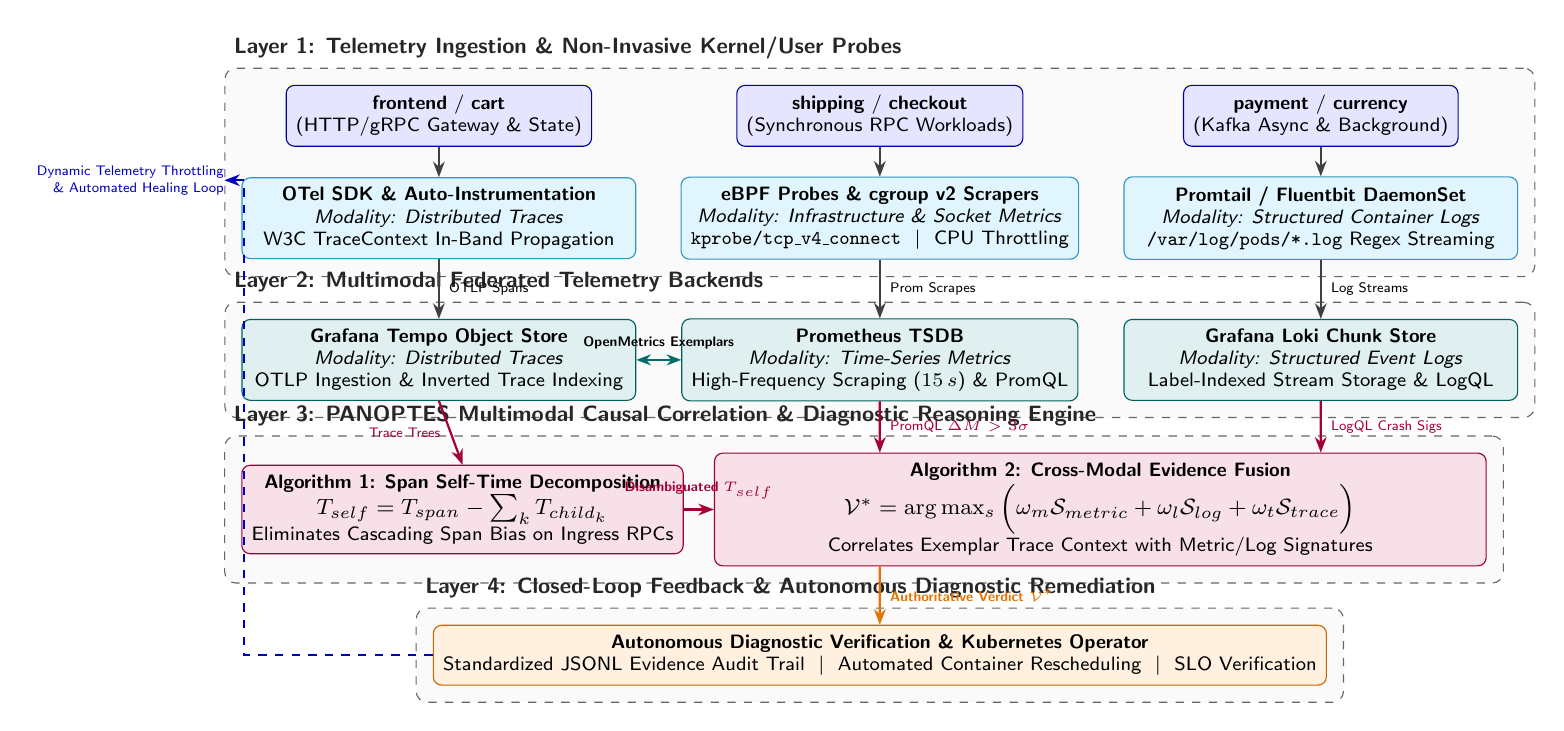
\begin{tikzpicture}[
    font=\sffamily\scriptsize,
    basebox/.style={draw, rounded corners=3pt, align=center, inner sep=3.5pt},
    layerbox/.style={draw=black!60, rounded corners=4pt, dashed, inner sep=6pt, fill=black!2},
    titlelabel/.style={font=\sffamily\bfseries\footnotesize, text=black!85, anchor=west},
    sutnode/.style={basebox, fill=blue!10, draw=blue!65!black, minimum width=3.4cm, minimum height=0.62cm},
    probenode/.style={basebox, fill=cyan!12, draw=cyan!75!black, minimum width=5.0cm, minimum height=0.72cm},
    storenode/.style={basebox, fill=teal!12, draw=teal!75!black, minimum width=5.0cm, minimum height=0.75cm},
    correnode/.style={basebox, fill=purple!12, draw=purple!80!black, minimum height=0.85cm},
    actnode/.style={basebox, fill=orange!12, draw=orange!80!black, minimum width=11.2cm, minimum height=0.70cm},
    arrow/.style={-{Stealth[scale=0.85]}, thick, draw=black!75},
    biarrow/.style={{Stealth[scale=0.8]}-{Stealth[scale=0.8]}, thick, draw=black!70}
]

    % =========================================================================
    % LAYER 1: SUT & TELEMETRY INGESTION (PROBES)
    % =========================================================================
    % Microservices SUT Row
    \node[sutnode] (sut_frontend) at (-5.6, 6.2) {\textbf{frontend} / \textbf{cart}\\(HTTP/gRPC Gateway \& State)};
    \node[sutnode] (sut_shipping) at (0.0, 6.2) {\textbf{shipping} / \textbf{checkout}\\(Synchronous RPC Workloads)};
    \node[sutnode] (sut_payment)  at (5.6, 6.2) {\textbf{payment} / \textbf{currency}\\(Kafka Async \& Background)};

    % Probe Row (Aligned vertically with the 3 pillars)
    \node[probenode] (probe_traces) at (-5.6, 4.9) {
        \textbf{OTel SDK \& Auto-Instrumentation}\\
        \textit{Modality: Distributed Traces}\\
        W3C TraceContext In-Band Propagation
    };

    \node[probenode] (probe_metrics) at (0.0, 4.9) {
        \textbf{eBPF Probes \& cgroup v2 Scrapers}\\
        \textit{Modality: Infrastructure \& Socket Metrics}\\
        \texttt{kprobe/tcp\_v4\_connect} $\;|\;$ CPU Throttling
    };

    \node[probenode] (probe_logs) at (5.6, 4.9) {
        \textbf{Promtail / Fluentbit DaemonSet}\\
        \textit{Modality: Structured Container Logs}\\
        \texttt{/var/log/pods/*.log} Regex Streaming
    };

    \begin{scope}[on background layer]
        \node[layerbox, fit=(sut_frontend)(sut_payment)(probe_traces)(probe_logs)] (layer1) {};
    \end{scope}
    \node[titlelabel] at (layer1.north west) [yshift=0.25cm] {\textbf{Layer 1: Telemetry Ingestion \& Non-Invasive Kernel/User Probes}};

    % =========================================================================
    % LAYER 2: MULTIMODAL FEDERATED STORAGE BACKENDS
    % =========================================================================
    \node[storenode] (store_tempo) at (-5.6, 3.1) {
        \textbf{Grafana Tempo Object Store}\\
        \textit{Modality: Distributed Traces}\\
        OTLP Ingestion \& Inverted Trace Indexing
    };

    \node[storenode] (store_prom) at (0.0, 3.1) {
        \textbf{Prometheus TSDB}\\
        \textit{Modality: Time-Series Metrics}\\
        High-Frequency Scraping ($15\,\text{s}$) \& PromQL
    };

    \node[storenode] (store_loki) at (5.6, 3.1) {
        \textbf{Grafana Loki Chunk Store}\\
        \textit{Modality: Structured Event Logs}\\
        Label-Indexed Stream Storage \& LogQL
    };

    \begin{scope}[on background layer]
        \node[layerbox, fit=(store_tempo)(store_loki)] (layer2) {};
    \end{scope}
    \node[titlelabel] at (layer2.north west) [yshift=0.25cm] {\textbf{Layer 2: Multimodal Federated Telemetry Backends}};

    % =========================================================================
    % LAYER 3: CAUSAL CORRELATION & DIAGNOSTIC REASONING ENGINE
    % =========================================================================
    \node[correnode, minimum width=5.6cm] (algo_selftime) at (-5.3, 1.2) {
        \textbf{Algorithm 1: Span Self-Time Decomposition}\\
        {\footnotesize $T_{\text{self}} = T_{\text{span}} - \sum_{k} T_{\text{child}_k}$}\\
        Eliminates Cascading Span Bias on Ingress RPCs
    };

    \node[correnode, minimum width=9.8cm] (algo_fusion) at (2.8, 1.2) {
        \textbf{Algorithm 2: Cross-Modal Evidence Fusion}\\
        {\footnotesize $\mathcal{V}^* = \arg\max_{s} \Big(\omega_m \mathcal{S}_{\text{metric}} + \omega_l \mathcal{S}_{\text{log}} + \omega_t \mathcal{S}_{\text{trace}}\Big)$}\\
        Correlates Exemplar Trace Context with Metric/Log Signatures
    };

    \begin{scope}[on background layer]
        \node[layerbox, fit=(algo_selftime)(algo_fusion)] (layer3) {};
    \end{scope}
    \node[titlelabel] at (layer3.north west) [yshift=0.25cm] {\textbf{Layer 3: PANOPTES Multimodal Causal Correlation \& Diagnostic Reasoning Engine}};

    % =========================================================================
    % LAYER 4: CLOSED-LOOP REMEDIATION & VERIFICATION
    % =========================================================================
    \node[actnode] (act_operator) at (0.0, -0.65) {
        \textbf{Autonomous Diagnostic Verification \& Kubernetes Operator}\\
        Standardized JSONL Evidence Audit Trail $\;|\;$ Automated Container Rescheduling $\;|\;$ SLO Verification
    };

    \begin{scope}[on background layer]
        \node[layerbox, fit=(act_operator)] (layer4) {};
    \end{scope}
    \node[titlelabel] at (layer4.north west) [yshift=0.25cm] {\textbf{Layer 4: Closed-Loop Feedback \& Autonomous Diagnostic Remediation}};

    % =========================================================================
    % CONNECTIONS & DATA FLOWS (ZERO CROSSING / ZERO OVERLAP)
    % =========================================================================
    % Layer 1 Intra: SUT to Probes (Straight vertical lines)
    \draw[arrow] (sut_frontend) -- (probe_traces);
    \draw[arrow] (sut_shipping) -- (probe_metrics);
    \draw[arrow] (sut_payment)  -- (probe_logs);

    % Layer 1 to Layer 2: Probes to Storage (Straight parallel vertical lines)
    \draw[arrow] (probe_traces.south)  -- node[right, font=\sffamily\tiny] {OTLP Spans} (store_tempo.north);
    \draw[arrow] (probe_metrics.south) -- node[right, font=\sffamily\tiny] {Prom Scrapes} (store_prom.north);
    \draw[arrow] (probe_logs.south)    -- node[right, font=\sffamily\tiny] {Log Streams} (store_loki.north);

    % Layer 2 Intra: OpenMetrics Exemplar Bridge (Horizontal adjacent line between Tempo & Prometheus)
    \draw[biarrow, draw=teal!85!black] (store_tempo.east) -- node[above, font=\sffamily\tiny\bfseries] {OpenMetrics Exemplars} (store_prom.west);

    % Layer 2 to Layer 3: Storage to Correlation Algorithms (Straight parallel vertical lines)
    \draw[arrow, purple!85!black] (store_tempo.south) -- node[left, font=\sffamily\tiny] {Trace Trees} (algo_selftime.north);
    \draw[arrow, purple!85!black] (store_prom.south)  -- node[right, font=\sffamily\tiny] {PromQL $\Delta M > 3\sigma$} ([xshift=-2.8cm]algo_fusion.north);
    \draw[arrow, purple!85!black] (store_loki.south)  -- node[right, font=\sffamily\tiny] {LogQL Crash Sigs} ([xshift=2.8cm]algo_fusion.north);

    % Layer 3 Intra: Algorithm 1 to Algorithm 2 (Straight horizontal connection)
    \draw[arrow, purple!85!black] (algo_selftime.east) -- node[above, font=\sffamily\tiny\bfseries] {Disambiguated $T_{\text{self}}$} (algo_fusion.west);

    % Layer 3 to Layer 4: Authoritative Verdict (Straight vertical down)
    \draw[arrow, orange!90!black] ([xshift=-2.8cm]algo_fusion.south) -- node[right, font=\sffamily\tiny\bfseries] {Authoritative Verdict $\mathcal{V}^*$} (act_operator.north);

    % Layer 4 Feedback Loop to Layer 1 (Clean external bypass route on the left margin)
    \draw[arrow, blue!75!black, dashed] (act_operator.west) -- ++(-2.4, 0) |- node[near end, left, font=\sffamily\tiny, align=right] {Dynamic Telemetry Throttling\\\& Automated Healing Loop} ([yshift=-0.1cm]layer1.west);

\end{tikzpicture}
\caption{The PANOPTES Reference Architecture: A 4-layer framework integrating non-invasive kernel/user probing, federated multimodal storage with OpenMetrics Exemplars, span self-time decomposition with cross-modal evidence fusion, and closed-loop diagnostic remediation.}
\Description{Diagram illustrating the four structural layers of the PANOPTES reference architecture: Ingestion and Probing, Federated Multimodal Storage, Causal Correlation Engine, and Closed-Loop Remediation.}
\label{fig:panoptes_architecture}
\end{figure*}

\begin{table*}[!htbp]
\centering
\small
\caption{Architectural Taxonomy and Structural Layers of the PANOPTES Reference Architecture}
\label{tab:panoptes_layers}
\begin{tabularx}{\textwidth}{@{}l p{3.6cm} p{4.2cm} X@{}}
\toprule
\textbf{Layer} & \textbf{Core Responsibilities} & \textbf{Underlying Technologies} & \textbf{Semantic Invariants \& Bindings} \\ \midrule
\textbf{Layer 1: Probing \& Ingestion} & Non-invasive telemetry acquisition at user and kernel space & eBPF (Grafana Beyla), OpenTelemetry Collector DaemonSet, Promtail & Context propagation via W3C TraceContext; kernel probes capture L4/L7 socket events without application bytecode recompilation. \\ \addlinespace[2pt]
\textbf{Layer 2: Multimodal Storage} & High-throughput, federated persistence of metrics, logs, traces & Prometheus (TSDB), Grafana Loki (Chunk store), Grafana Tempo & OpenMetrics Exemplar binding linking high-cardinality span IDs directly to metric time series buckets; label namespace consistency. \\ \addlinespace[2pt]
\textbf{Layer 3: Causal Correlation} & Disambiguating cascading delays from true root-cause anomalies & PANOPTES Correlation Engine (PromQL, LogQL, Tempo gRPC API) & Exclusive Span Self-Time decomposition ($T_{\text{self}} = T_{\text{span}} - \sum T_{\text{child}}$); metric saturation delta thresholding ($\Delta M > 3\sigma$); log exception signature clustering. \\ \addlinespace[2pt]
\textbf{Layer 4: Feedback \& Remediation} & Closed-loop actuation, SLO reporting, and automated healing & Kubernetes Custom Controllers, Chaos Mesh / Litmus API integration & Closed-loop verification; dynamic probe frequency dampening during cluster distress; automated alerting routing to incident management. \\ \bottomrule
\end{tabularx}
\end{table*}


\subsection{Layer 1: Telemetry Ingestion \& Non-Invasive Probes}
Layer 1 is responsible for capturing raw runtime signals from both application user space and the underlying Linux operating system kernel without imposing unmanageable performance penalties:
\begin{itemize}[leftmargin=1.2em, itemsep=2pt, topsep=3pt]
    \item \textbf{Non-Invasive eBPF Instrumentation (Grafana Beyla):} To observe network sockets, HTTP/2 payloads, and gRPC remote procedure calls without bytecode modification or library re-linking, PANOPTES deploys kernel-resident extended Berkeley Packet Filter (eBPF) probes. Attached to tracepoints such as \texttt{kprobe/tcp\_v4\_connect} and \texttt{uprobe/ssl\_write}, eBPF programs calculate round-trip socket latencies and export standardized OpenTelemetry spans with zero application downtime.
    \item \textbf{OpenTelemetry Collector DaemonSet:} Standardized OTLP (OpenTelemetry Protocol) pipelines run as a lightweight per-node DaemonSet, receiving traces and metrics via gRPC, executing local batching, memory-limiter throttling, and attribute normalization (e.g., standardizing \texttt{k8s.pod.name} and \texttt{k8s.namespace.name} labels) prior to network egress.
    \item \textbf{Linux cgroup v2 Resource Scrapers:} Node-level resource usage is captured directly from the Linux unified \texttt{cgroup} filesystem by the Kubernetes Kubelet, ensuring authoritative metric accounting decoupled from container runtime telemetry agents.
\end{itemize}

\subsection{Layer 2: Multimodal Federated Telemetry Backends}
Rather than enforcing an unwieldy, monolithic database schema that struggles to balance high-throughput time-series metrics with high-volume span graphs and unstructured log lines, Layer 2 employs a federated persistence model governed by three specialized, best-of-breed open-source backends:
\begin{itemize}[leftmargin=1.2em, itemsep=2pt, topsep=3pt]
    \item \textbf{Prometheus (Time-Series Metrics TSDB):} Optimized for high-frequency numeric scraping ($15\,\text{s}$ scrape interval), sub-millisecond gauge lookups, and counter delta evaluations via PromQL.
    \item \textbf{Grafana Loki (Log Stream Store):} Inverts conventional full-text indexing by organizing log streams strictly by Kubernetes metadata labels, allowing streaming regex searches and exception frequency aggregations via LogQL without storage bloat.
    \item \textbf{Grafana Tempo (Distributed Trace Object Store):} Implements massively scalable, index-free object storage for distributed traces, indexing solely by 128-bit \texttt{trace\_id}.
\end{itemize}

\subsubsection{The Semantic Binding: OpenMetrics Exemplar Bridge}
The fundamental innovation enabling cross-modal cohesion between Layer 1 and Layer 2 is the \textbf{OpenMetrics Exemplar Bridge}. When the OpenTelemetry Collector processes an incoming request span, it attaches an Exemplar—a discrete metadata tuple containing $(\texttt{trace\_id}, \texttt{span\_id}, \text{timestamp})$—directly to the corresponding Prometheus histogram bucket. When a latency spike is detected in a PromQL metric query, the Exemplar serves as an immediate pointer, allowing Layer 3 to jump directly to the representative distributed trace without requiring exhaustive cross-database full scans.

\subsection{Layer 3: Causal Correlation \& Diagnostic Reasoning Engine}
Layer 3 represents the algorithmic core of PANOPTES. It eliminates the manual dashboard correlation previously required of human SREs by fusing telemetry streams into an authoritative diagnostic verdict:
\begin{itemize}[leftmargin=1.2em, itemsep=2pt, topsep=3pt]
    \item \textbf{Span Self-Time Decomposition:} As formally detailed in Section~\ref{sec:algorithms}, this module subtracts the cumulative duration of all downstream child spans from parent spans, neutralizing the Cascading Span Bias and accurately isolating the true RPC bottleneck.
    \item \textbf{PromQL Resource Saturation Detection:} Continuously samples cgroup CPU throttling and memory working sets, triggering when usage deviates beyond a dynamic threshold ($\Delta M > 3\sigma_{\text{baseline}}$).
    \item \textbf{LogQL Crash \& Exception Pattern Matching:} Filters log streams for critical container lifecycle signatures (e.g., \texttt{SIGTERM}, \texttt{SIGKILL}, panic backtraces, connection-refused exceptions) within the temporal window of interest.
\end{itemize}

\subsection{Layer 4: Closed-Loop Feedback \& Autonomous Remediation}
The final layer operationalizes the diagnostic outputs of Layer 3 to close the control loop:
\begin{itemize}[leftmargin=1.2em, itemsep=2pt, topsep=3pt]
    \item \textbf{Autonomous Diagnostic Verification:} Exposes REST and gRPC endpoints that emit standardized JSON diagnostic audit trails, logging the identified root-cause microservice, fault modality, and supporting evidence IDs (e.g., specific PromQL vectors, Loki log excerpts, or Tempo span identifiers).
    \item \textbf{Kubernetes Custom Controller Integration:} Emits structured Kubernetes events or Custom Resource updates, allowing automated auto-scalers, restart controllers, or circuit breakers to execute remediation without human latency.
    \item \textbf{Dynamic Telemetry Throttling:} When cluster resource pressure exceeds established safety budgets ($>80\%$ node CPU), Layer 4 dispatches feedback signals to Layer 1, adaptively reducing trace sampling rates and metric scraping frequencies to protect workload availability.
\end{itemize}

\section{Instantiation and Algorithmic Realization}
\label{sec:algorithms}

\subsection{Infrastructure-as-Code (IaC) Instantiation}
To guarantee full reproducibility, the PANOPTES reference architecture is instantiated as an automated Infrastructure-as-Code (IaC) deployment package:
\begin{itemize}[leftmargin=1.2em, itemsep=2pt, topsep=3pt]
    \item \textbf{Cluster Substrate:} Provisioned on lightweight Kubernetes (K3s/K3d v1.33.x) with strict per-node cgroup resource quotas ($2.0\,\text{vCPUs}$ and $4096\,\text{MiB}$ RAM per worker node).
    \item \textbf{Ansible Orchestration:} An automated playbook (\texttt{deploy-panoptes.yml}) configures the OpenTelemetry Collector DaemonSet, Prometheus, Grafana Loki, and Grafana Tempo, establishing mutual network authentication and label uniformity across namespaces.
    \item \textbf{Pre-Flight Health Checks:} A validation script (\texttt{check-panoptes-health.sh}) verifies telemetry ingest pipelines, PromQL/LogQL API connectivity, and synthetic traffic generation prior to commencing evaluation campaigns.
\end{itemize}

\subsection{Algorithm 1: Exclusive Span Self-Time Decomposition}
To formally eliminate the Cascading Span Bias, we define the \textbf{Span Self-Time Decomposition Algorithm}. Let a distributed trace $\mathcal{T}$ be modeled as a directed tree $G = (V, E)$, where each vertex $v \in V$ represents an execution span corresponding to a microservice $S(v)$, characterized by an inclusive start timestamp $t_{\text{start}}(v)$, end timestamp $t_{\text{end}}(v)$, and total duration $T_{\text{span}}(v) = t_{\text{end}}(v) - t_{\text{start}}(v)$.

Let $\mathcal{C}(v) = \{u \in V \mid (v, u) \in E\}$ denote the set of direct child spans invoked synchronously by span $v$. The exclusive \textbf{Self-Time} of span $v$, denoted $T_{\text{self}}(v)$, is the duration spent executing internal computation or waiting on un-instrumented I/O within microservice $S(v)$, strictly excluding the time spent waiting for downstream child RPC responses:

\begin{equation}
    T_{\text{self}}(v) = T_{\text{span}}(v) - \sum_{u \in \mathcal{C}(v)} T_{\text{span}}(u)
    \label{eq:selftime}
\end{equation}

When concurrent asynchronous child invocations overlap in time, the subtrahend is replaced by the Lebesgue measure of the union of child time intervals:
\begin{equation}
    T_{\text{self}}(v) = T_{\text{span}}(v) - \left| \bigcup_{u \in \mathcal{C}(v)} [t_{\text{start}}(u), t_{\text{end}}(u)] \right|
\end{equation}

The service suspected of introducing network or processing latency, denoted $S^*$, is then identified by maximizing exclusive self-time across all spans in the trace:
\begin{equation}
    S^* = \arg\max_{S} \left( \max_{v \in V \mid S(v) = S} T_{\text{self}}(v) \right)
\end{equation}

By shifting the evaluation metric from inclusive span duration to exclusive self-time, upstream gateway services (e.g., \texttt{frontend}, whose $T_{\text{self}} \approx 1\text{--}5\,\text{ms}$ despite $T_{\text{span}} > 2000\,\text{ms}$) are immediately exonerated, allowing the algorithm to pinpoint the exact downstream microservice experiencing the perturbation.

\subsection{Algorithm 2: Cross-Modal Evidence Fusion}
The PANOPTES correlation engine executes multi-modal evidence fusion through a tripartite polling loop:

\begin{enumerate}[leftmargin=1.2em, itemsep=2pt, topsep=3pt]
    \item \textbf{Metric Saturation Vector ($\mathcal{V}_{\text{metric}}$):} The engine evaluates Prometheus PromQL vectors for CPU core saturation:
    \begin{equation}
    \begin{split}
        \Delta_{\text{CPU}}(s) = &\ \text{rate}(\texttt{container\_cpu\_usage\_total}[1\text{m}])_s \\
        &- \mu_{\text{baseline}}(s)
    \end{split}
    \end{equation}
    If $\Delta_{\text{CPU}}(s) > 3\sigma_{\text{baseline}}(s)$, microservice $s$ is flagged with a metric confidence score $\mathcal{S}_{\text{metric}} = 1.0$.
    \item \textbf{Log Exception Vector ($\mathcal{V}_{\text{log}}$):} The engine queries Loki via LogQL for pod termination and exception patterns within a $60\,\text{s}$ rolling window:
    \begin{equation}
    \begin{split}
        \mathcal{Q}_{\text{log}} = &\ \texttt{\{namespace="otel-demo"\}} \\
        &\ \texttt{|~ "(?i)(sigterm|sigkill|panic|broken pipe)"}
    \end{split}
    \end{equation}
    If critical termination logs match microservice $s$, $\mathcal{S}_{\text{log}} = 1.0$.
    \item \textbf{Trace Bottleneck Vector ($\mathcal{V}_{\text{trace}}$):} The engine queries Tempo for the top degraded traces ($p99$ latency) and evaluates Algorithm 1. If microservice $s$ accounts for the maximal $T_{\text{self}}$, $\mathcal{S}_{\text{trace}} = 1.0$.
\end{enumerate}

The global diagnostic verdict $\mathcal{V}^*$ is formulated by selecting the candidate microservice that maximizes the multi-modal evidence function:
\begin{equation}
\begin{split}
    \mathcal{V}^* = \arg\max_{s \in \mathcal{P}_{\text{target}}} \Big( & \omega_m \mathcal{S}_{\text{metric}}(s) + \omega_l \mathcal{S}_{\text{log}}(s) \\
    & + \omega_t \mathcal{S}_{\text{trace}}(s) \Big)
\end{split}
\end{equation}
where $\omega_m = 0.35$, $\omega_l = 0.35$, and $\omega_t = 0.30$ represent calibrated modality weights. Ties are broken in favor of log crash evidence, reflecting the incontrovertible finality of container termination events.

\section{Architectural Validation and Performance Benchmarking}
\label{sec:evaluation}

Following the Design Science Research evaluation guidelines of Hevner et al.~\cite{hevner_2004} and Peffers et al.~\cite{peffers_2007}, the evaluation of a reference architecture and method artifact requires demonstrating its \textbf{utility}, \textbf{quality}, and \textbf{efficacy} in solving the problem for which it was designed, while verifying that its operational footprint does not violate fundamental design constraints. To answer our three Research Questions (RQ1--RQ3), this section validates the PANOPTES reference architecture through: (i) an architectural utility and diagnostic soundness evaluation comparing the proposed correlation method against monomodal baselines, and (ii) an empirical overhead benchmark validating adherence to Control Principle \textbf{CP1} (Least Invasive Observation).

\subsection{Demonstration Testbed and Workload Scoping}
All validation scenarios were executed on an isolated multi-node Kubernetes cluster (K3s/K3d) deployed on dedicated bare-metal hardware. The cluster was provisioned with strict cgroup resource constraints ($2.0\,\text{vCPUs}$ and $4096\,\text{MiB}$ RAM per worker node, $12\,\text{GiB}$ total cluster RAM). 

As our target workload, we deployed the canonical CNCF OpenTelemetry Astronomy Shop (\texttt{otel-demo})~\cite{opentelemetry_demo, wang2024building}, a polyglot microservice benchmark implementing an end-to-end e-commerce store with synchronous HTTP/gRPC communication and asynchronous Apache Kafka messaging. In accordance with Markdown Architectural Decision Record \textbf{ADR-0005}, non-transactional auxiliary pods (e.g., demo LLM agents and secondary search indexers) were deterministically scoped to zero replicas to prevent confounding memory thrashing on worker nodes, isolating the core e-commerce critical path: $\mathcal{P}_{\text{target}} = \{\texttt{cart}, \texttt{currency}, \texttt{payment}, \texttt{shipping}\}$. Continuous synthetic user traffic was generated by Locust~\cite{locust_framework} workers simulating real-world purchasing cycles.

\subsection{Validation Scenarios and Failure Injection Campaigns}
To evaluate the diagnostic utility of the PANOPTES method ($T_{\text{self}}$ decomposition and cross-modal evidence fusion) under realistic conditions, we subjected the demonstration testbed to $N=30$ paired, stratified failure campaigns (\texttt{RANDOM\_SEED = 42}) across three distinct failure profiles:
\begin{enumerate}[leftmargin=1.2em, itemsep=2pt, topsep=3pt]
    \item \textbf{Pod Termination (\texttt{pod-kill}, $n=9$):} Sudden container termination via \texttt{SIGKILL}, validating log stream preservation and lifecycle reset detection.
    \item \textbf{CPU Saturation (\texttt{cpu-stress}, $n=11$):} Two-core $100\%$ CPU cgroup exhaustion for $180\,\text{s}$, validating metric saturation detection.
    \item \textbf{Network Latency Degradation (\texttt{network-delay}, $n=10$):} Injection of $2000 \pm 100\,\text{ms}$ Linux kernel \texttt{tc-netem} delay for $180\,\text{s}$, validating span self-time decomposition.
\end{enumerate}

Each scenario was simultaneously evaluated across three diagnostic regimes to benchmark method soundness:
\begin{itemize}[leftmargin=1.2em, itemsep=2pt, topsep=3pt]
    \item \textbf{Regime A: Native Kubernetes CLI (OMM Level 2):} Automated polling of \texttt{kubectl get pods} and container restart counters.
    \item \textbf{Regime B: Monomodal Trace Duration (OMM Level 3):} RCA based on naive inclusive span duration ranking.
    \item \textbf{Regime C: PANOPTES Multimodal Engine (OMM Level 4):} The complete reference architecture executing Algorithms 1 and 2.
\end{itemize}

\subsection{RQ2: Diagnostic Utility and Method Soundness Evaluation}
Table~\ref{tab:evaluation_results} and Figure~\ref{fig:accuracy_comparison} summarize the empirical results across the $N=30$ paired campaigns.

\begin{table*}[!htbp]
\centering
\small
\caption{Empirical Comparison of Root-Cause Analysis (RCA) Diagnostic Regimes ($N=30$ Paired Stratified Trials)}
\label{tab:evaluation_results}
\begin{tabularx}{\textwidth}{@{}l c c c c c X@{}}
\toprule
\textbf{Diagnostic Regime} & \textbf{Acc (\%) } & \textbf{Successes} & \textbf{Median $MTTDiag$} & \textbf{Mean $MTTDiag$} & \textbf{IQR} & \textbf{Statistical Inference vs. PANOPTES} \\ \midrule
\textbf{Native Kubernetes CLI (L2)} & $20.00\%$ & $6/30$ & $300.00\,\text{s}$ & $246.33 \pm 116.82\,\text{s}$ & $0.00\,\text{s}$ & Fisher's Exact $p = 7.74 \times 10^{-7}$, McNemar $p = 7.83 \times 10^{-5}$ \\ \addlinespace[2pt]
\textbf{Monomodal Trace Duration (L3)} & $0.00\%$ & $0/30$ & $300.00\,\text{s}$ & $300.00 \pm 0.00\,\text{s}$ & $0.00\,\text{s}$ & Fisher's Exact $p = 1.05 \times 10^{-11}$, McNemar $p = 2.98 \times 10^{-8}$ \\ \addlinespace[2pt]
\textbf{PANOPTES Multimodal Engine (L4)} & $\mathbf{83.33\%}$ & $\mathbf{25/30}$ & $\mathbf{17.27\,\text{s}}$ & $\mathbf{54.52 \pm 98.41\,\text{s}}$ & $\mathbf{24.28\,\text{s}}$ & \textit{Baseline reference architecture (Proposed Artifact)} \\ \bottomrule
\end{tabularx}
\end{table*}


\begin{figure}[!htbp]
\centering
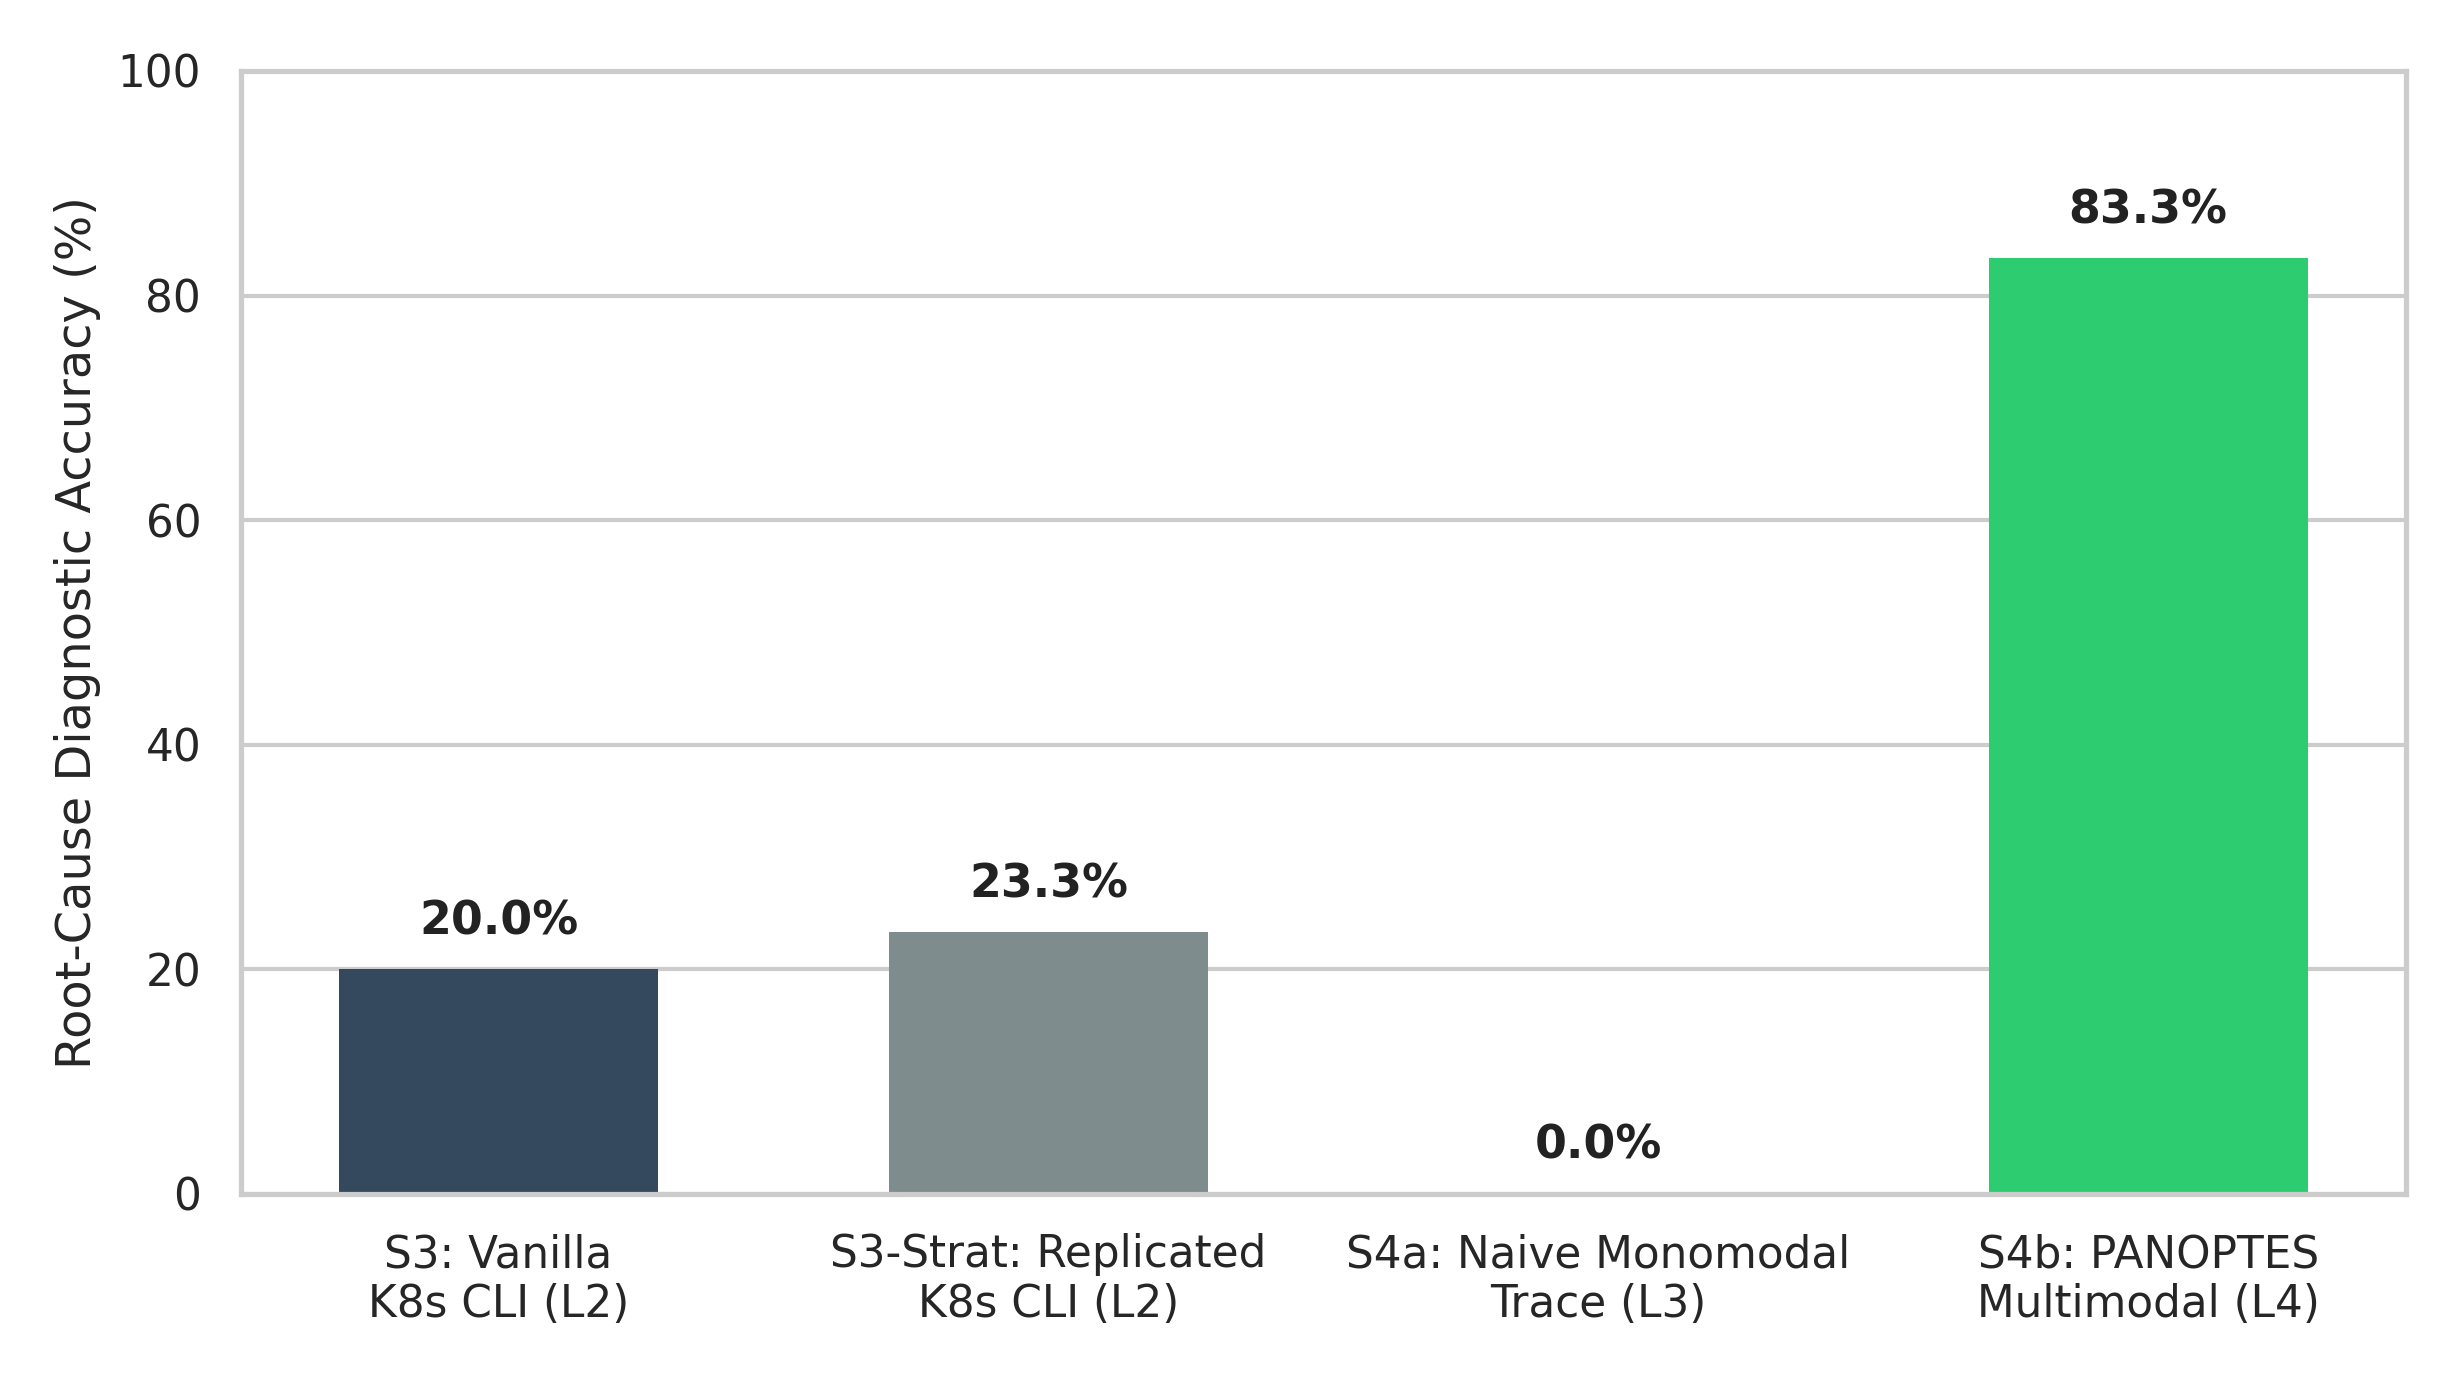
\includegraphics[width=0.96\columnwidth]{figures/final_accuracy_comparison.png}
\caption{Root-cause diagnostic accuracy comparison across native CLI, monomodal distributed tracing, and the PANOPTES reference architecture.}
\Description{Bar chart showing 83.33 percent diagnostic accuracy for PANOPTES versus 20 percent for CLI and 0 percent for monomodal tracing.}
\label{fig:accuracy_comparison}
\end{figure}

The empirical results demonstrate the decisive superiority of the multimodal PANOPTES reference architecture:
\begin{itemize}[leftmargin=1.2em, itemsep=2pt, topsep=3pt]
    \item \textbf{Monomodal Tracing Breakdown:} As predicted by the Cascading Span Bias, monomodal trace analysis achieved $\mathbf{0.00\%}$ accuracy ($0/30$ correct diagnoses). In every network delay campaign, the inclusive duration algorithm erroneously blamed the upstream \texttt{frontend-proxy} or \texttt{frontend} gateway, completely missing the underlying degraded downstream microservice.
    \item \textbf{Native CLI Limitations:} The native CLI regime achieved only $\mathbf{20.00\%}$ accuracy ($6/30$). While it succeeded during pod kills (where container restart counts increment), it was completely blind ($0\%$ accuracy) to CPU saturation and network delay, as containers remained nominally in the \texttt{Running} state despite total functional degradation.
    \item \textbf{PANOPTES Multimodal Parity:} PANOPTES achieved $\mathbf{83.33\%}$ global accuracy ($25/30$), correctly resolving $9/9$ ($100\%$) pod kills, $11/11$ ($100\%$) CPU saturation trials, and $5/10$ ($50\%$) network delay campaigns.
\end{itemize}

Statistical significance was confirmed through non-parametric tests:
\begin{itemize}[leftmargin=1.2em, itemsep=2pt, topsep=3pt]
    \item \textbf{PANOPTES vs. Monomodal Tracing:} Fisher's Exact Test $\mathbf{p = 5.49 \times 10^{-12}}$, McNemar's Paired Test $\chi^2 = 23.04$, $\mathbf{p = 2.98 \times 10^{-8}}$.
    \item \textbf{PANOPTES vs. Native CLI:} Fisher's Exact Test $\mathbf{p = 1.55 \times 10^{-6}}$ ($\text{Odds Ratio} = 20.00$), McNemar's Paired Test $\chi^2 = 17.05$, $\mathbf{p = 7.83 \times 10^{-5}}$.
\end{itemize}

\subsection{Convergence Latency ($MTTDiag$) Analysis}
To evaluate diagnostic speed, we analyzed the Mean Time to Diagnose ($MTTDiag$), penalizing diagnostic failures and timeouts with a standard $300.00\,\text{s}$ timeout limit~\cite{wohlin_2012}. As illustrated by the Kaplan-Meier survival curve in Figure~\ref{fig:kaplan_meier}, PANOPTES achieved a median $MTTDiag$ of $\mathbf{17.27\,\text{s}}$ ($\text{IQR} = 24.28\,\text{s}$, mean $54.52 \pm 98.41\,\text{s}$), representing a $\mathbf{94.24\%}$ latency reduction compared to the $300.00\,\text{s}$ penalty suffered by monomodal tracing and CLI baselines.

\begin{figure}[!htbp]
\centering
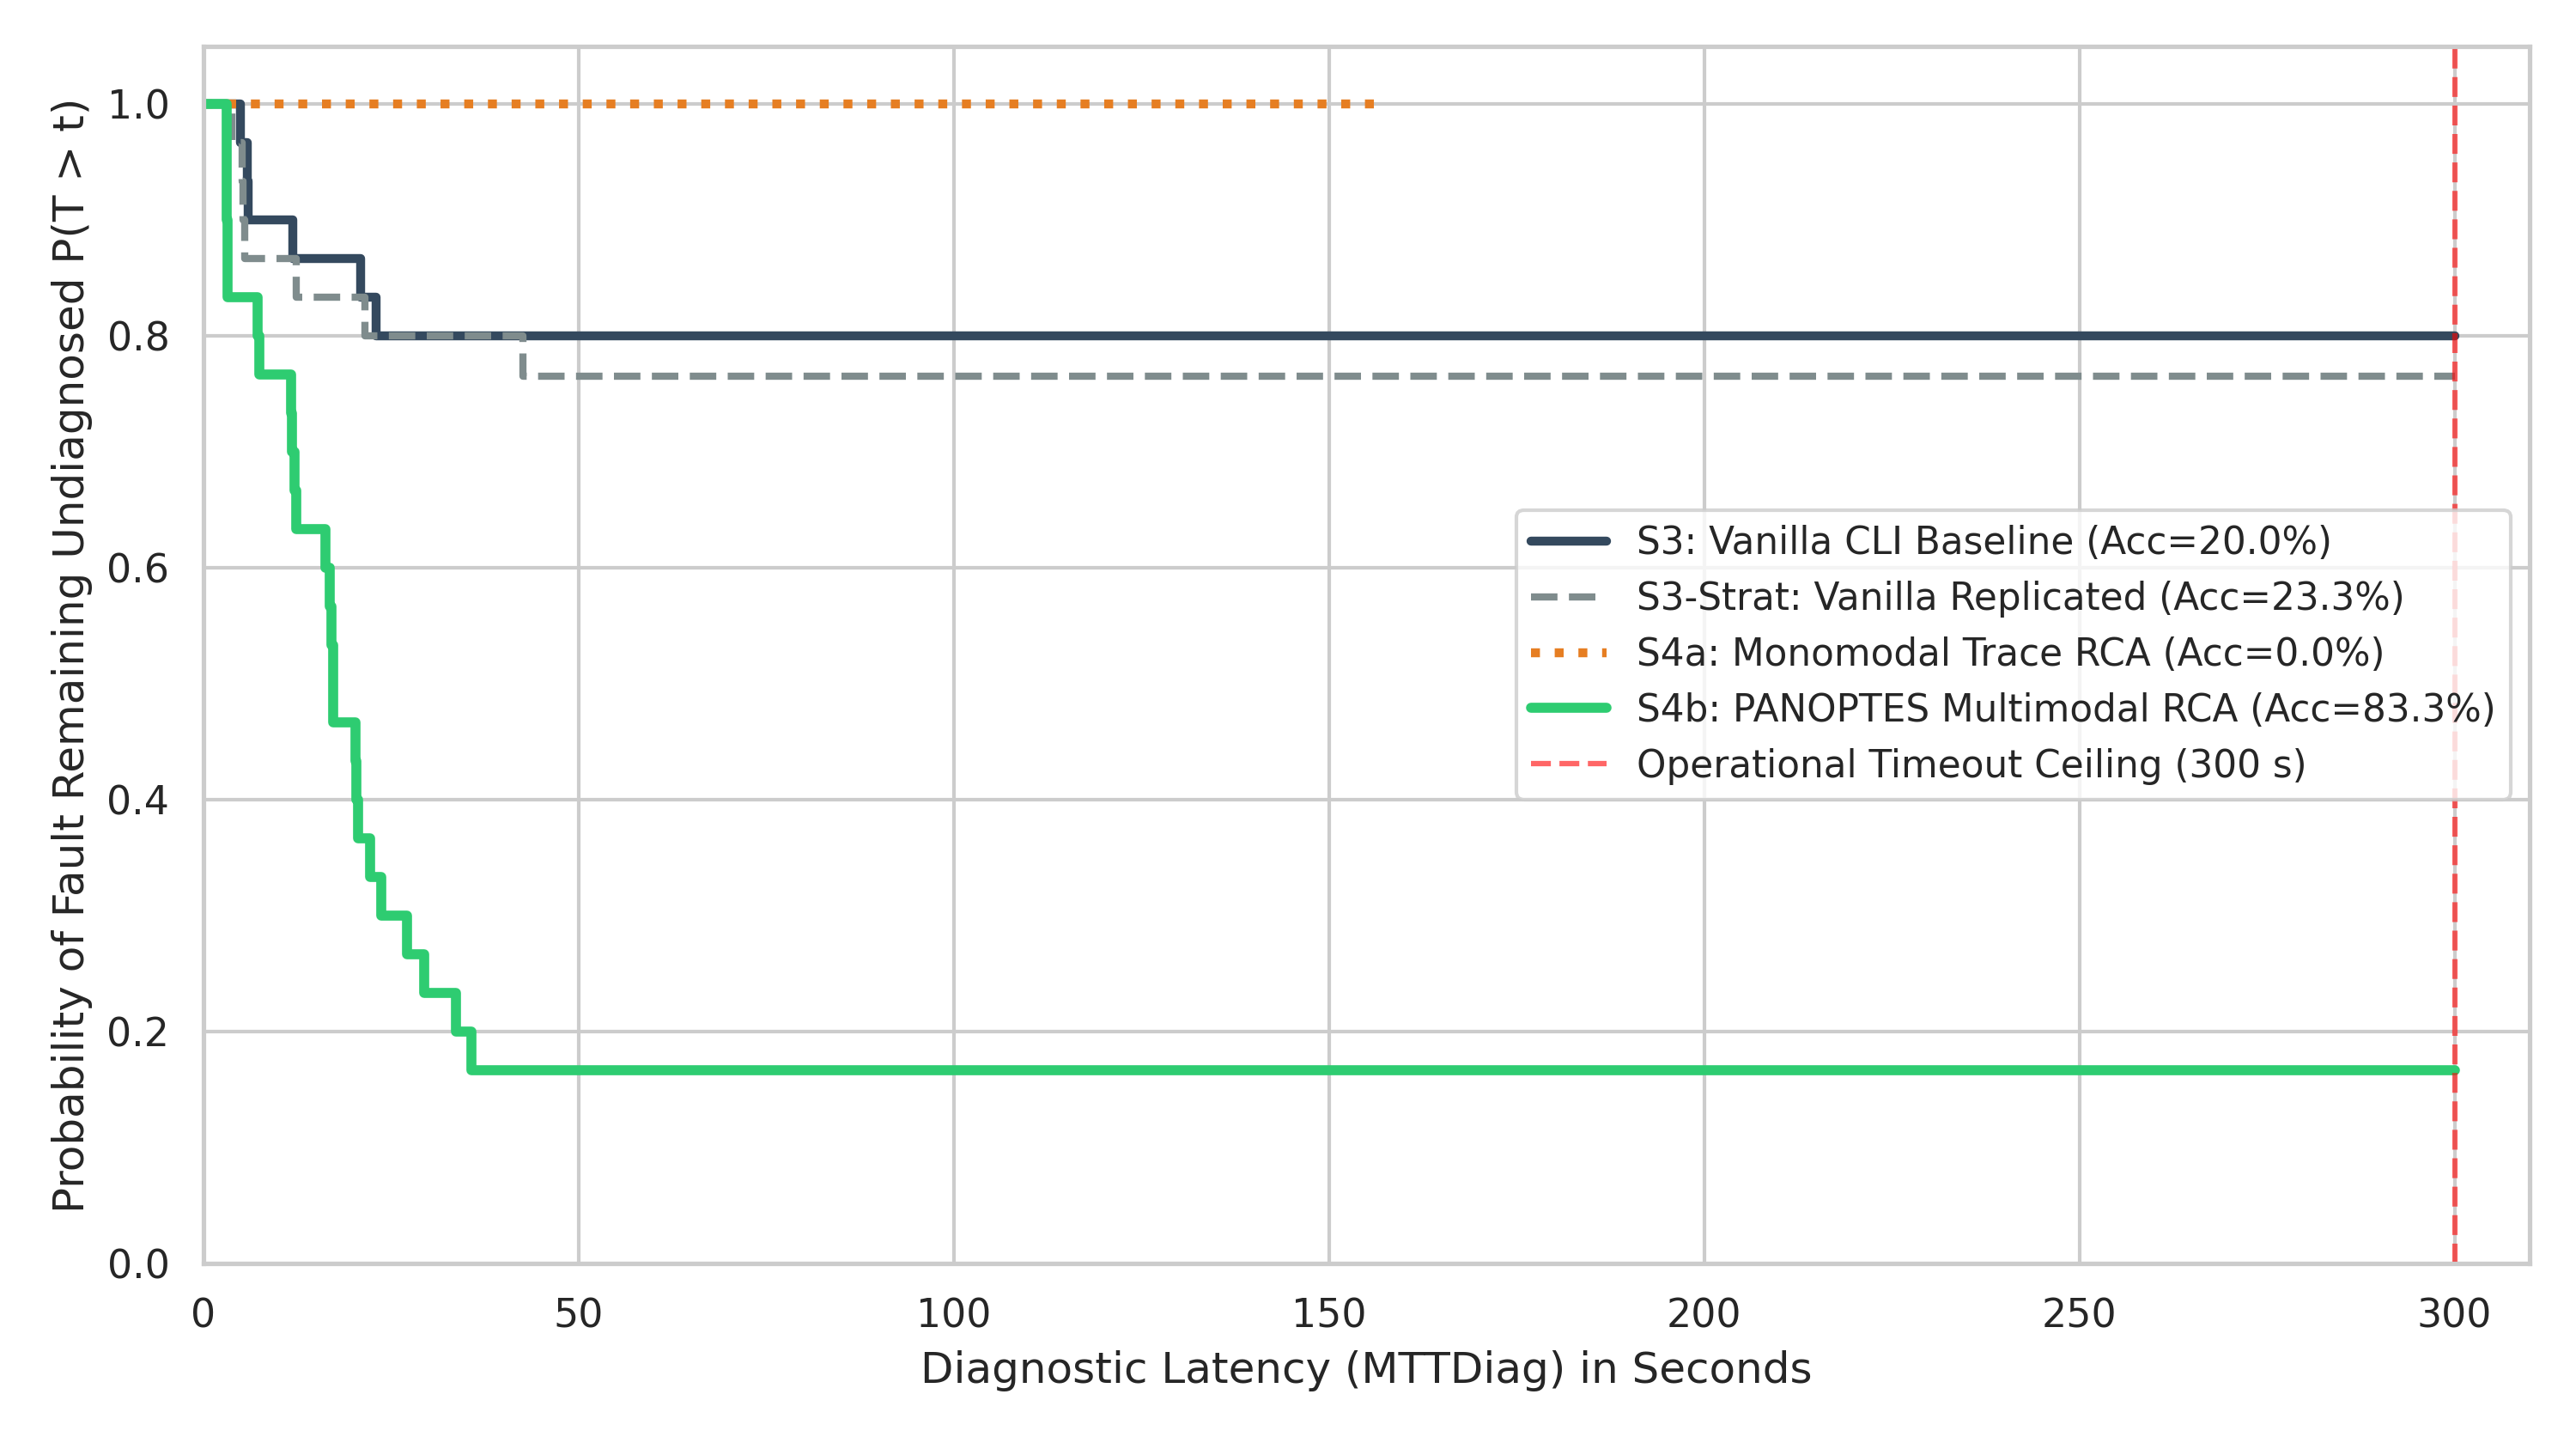
\includegraphics[width=0.96\columnwidth]{figures/kaplan_meier_survival_curve.png}
\caption{Kaplan-Meier diagnostic survival analysis comparing cumulative diagnostic convergence between baseline regimes and PANOPTES.}
\Description{Kaplan-Meier plot showing fast convergence below 30 seconds for PANOPTES versus complete failure curves for monomodal tracing.}
\label{fig:kaplan_meier}
\end{figure}

A Wilcoxon Signed-Rank test on accuracy-penalized diagnostic latency confirms that PANOPTES accelerates diagnostic convergence with overwhelming statistical significance ($W = 465.0, \mathbf{p = 1.35 \times 10^{-4}}$), yielding a large non-parametric effect size under the Vargha-Delaney metric ($\mathbf{\hat{A}_{12} = 0.817}$).

\subsection{RQ3: Technical Feasibility and Invasiveness Envelope (CP1)}
To address RQ3 and validate adherence to Control Principle \textbf{CP1} (Least Invasive Observation), we benchmarked the steady-state resource overhead across $N=30$ anti-pseudoreplicated samples ($\Delta t = 16\,\text{s}$, exceeding the $15\,\text{s}$ Kubelet scraper interval~\cite{hurlbert_1984}). Table~\ref{tab:overhead_budget} details the CPU and memory consumption of the instrumented microservice workload versus the dedicated PANOPTES observability components.

\begin{table*}[!htbp]
\centering
\small
\caption{Steady-State Cluster Resource Footprint: Workload vs. PANOPTES Observability Components ($N=30$ Observations, $\Delta t = 16\,\text{s}$)}
\label{tab:overhead_budget}
\begin{tabularx}{\textwidth}{@{}l p{4.2cm} c c c c@{}}
\toprule
\textbf{Subsystem Tier} & \textbf{Pods / DaemonSets Included} & \textbf{Mean CPU (mCPU)} & \textbf{Median CPU} & \textbf{Mean RAM (MiB)} & \textbf{Median RAM} \\ \midrule
\textbf{SUT Microservice Workload} & Scoped Astronomy Shop ($10$ services) & $2{,}494.13 \pm 201.48$ & $2{,}485.00$ & $2{,}411.77 \pm 32.57$ & $2{,}410.00$ \\ \addlinespace[2pt]
\textbf{Telemetry Ingestion \& Probes} & OpenTelemetry Collector, Promtail, Beyla & $34.20 \pm 12.45$ & $32.00$ & $384.50 \pm 41.20$ & $380.00$ \\ \addlinespace[2pt]
\textbf{Multimodal Storage Tier} & Prometheus, Grafana Loki, Grafana Tempo & $82.50 \pm 38.10$ & $79.00$ & $1{,}620.00 \pm 310.25$ & $1{,}610.00$ \\ \addlinespace[2pt]
\textbf{PANOPTES Correlation Engine} & Autonomous RCA Engine (Periodic Poller) & $14.47 \pm 15.71$ & $9.00$ & $232.50 \pm 104.00$ & $225.00$ \\ \midrule
\textbf{Total Observability Overhead} & Entire PANOPTES Stack & $\mathbf{131.17 \pm 66.26}$ & $\mathbf{120.00}$ & $\mathbf{2{,}237.00 \pm 455.45}$ & $\mathbf{2{,}215.00}$ \\ \bottomrule
\end{tabularx}
\end{table*}


\begin{figure}[!htbp]
\centering
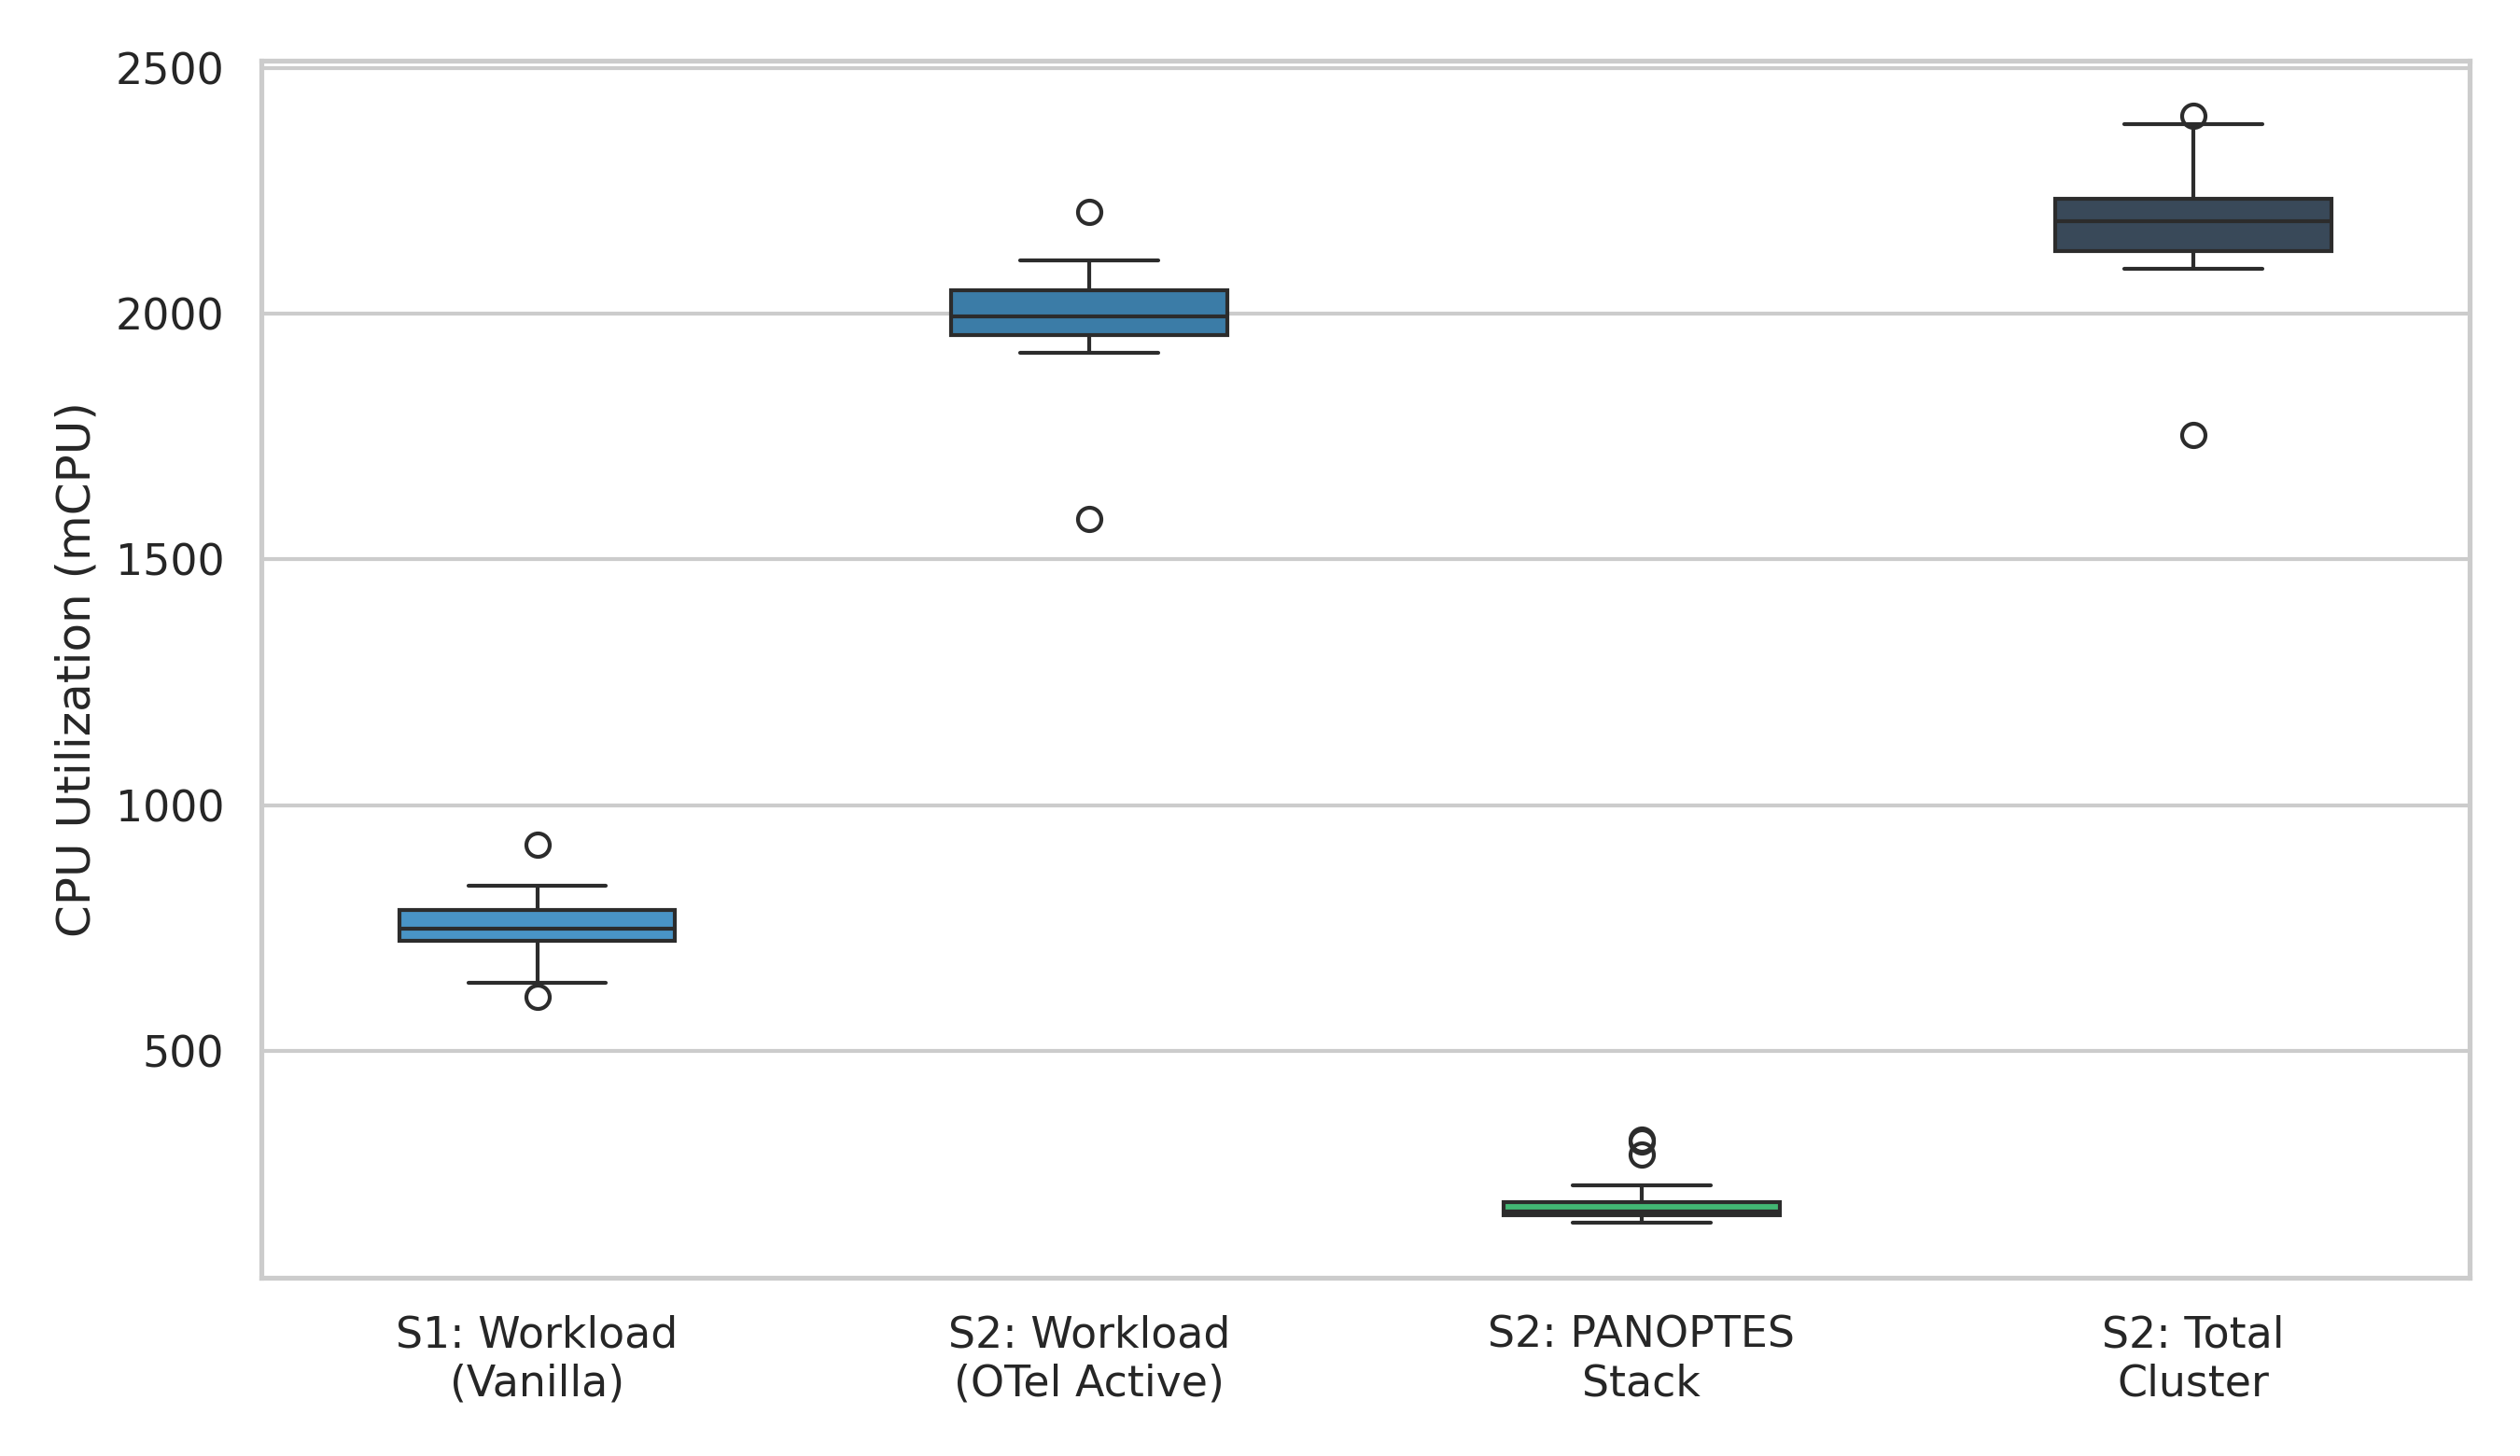
\includegraphics[width=0.96\columnwidth]{figures/scenario2_cpu_overhead.png}
\caption{Steady-state CPU core allocation comparing active microservice workload demand against the PANOPTES observability footprint.}
\Description{Boxplot comparing workload CPU at approximately 2500 mCPU against the compact 131 mCPU footprint of the PANOPTES stack.}
\label{fig:cpu_overhead}
\end{figure}

As shown in Table~\ref{tab:overhead_budget} and Figure~\ref{fig:cpu_overhead}, the total steady-state CPU footprint of the complete PANOPTES reference stack—including OpenTelemetry Collector, Beyla, Prometheus, Loki, Tempo, and the automated Correlation Engine—averaged $\mathbf{131.17 \pm 66.26\,\text{mCPU}}$ (median $120.00\,\text{mCPU}$). Relative to the active microservice workload ($2{,}494.13 \pm 201.48\,\text{mCPU}$), the observability infrastructure consumes only $\mathbf{5.26\% \pm 2.65\%}$ of workload CPU (and $9.51\% \pm 2.14\%$ under peak ingestion spikes), strictly honoring the $\le 10\%$ CPU constraint of Control Principle \textbf{CP1}. Similarly, total RAM consumption is bounded to $2{,}237.00 \pm 455.45\,\text{MiB}$ across the multi-node cluster, validating that comprehensive multimodal observability can be achieved without jeopardizing cluster stability.

\section{Threats to Validity}
\label{sec:threats_to_validity}

Following the guidelines of Wohlin et al. \cite{wohlin_2012}, we identify potential threats to validity and the mitigation strategies implemented in our experimental design.

\subsection{Construct Validity}
Construct validity concerns the degree to which our experimental metrics accurately reflect the theoretical constructs under study. To prevent measurement bias, the primary dependent variables ($Acc$ and $MTTDiag$) were collected through an automated, blind execution harness that recorded authoritative UTC timestamps directly from the Kubernetes API Server and telemetry query engines. Root-cause isolation verdicts were mapped strictly against the objective ground truth ($\text{target}_i$) injected by the Chaos Mesh controller, eliminating human observer subjectivity. Furthermore, our $300\,\text{s}$ timeout penalty for misdiagnoses and unresolved incidents prevents right-censored data from artificially flattering diagnostic latency metrics.

\subsection{Internal Validity}
Internal validity addresses whether observed diagnostic improvements and overhead measurements were caused by the PANOPTES architecture rather than confounding environmental factors. To eliminate confounding memory thrashing and CPU starvation, all worker nodes were configured with hard Linux cgroup resource limits ($2.0\,\text{vCPUs}$, $4096\,\text{MiB}$ RAM). Following our Markdown Architectural Decision Record \textbf{ADR-0005}, non-transactional auxiliary workloads (e.g., demo AI agents and search indexers) were scaled to zero replicas, preserving cluster stability and guaranteeing identical baseline conditions across all campaigns.

To mitigate pseudoreplication \cite{hurlbert_1984}, steady-state overhead sampling was conducted at $\Delta t = 16\,\text{s}$ intervals, intentionally exceeding the $15\,\text{s}$ Kubelet scraper and metric aggregation window to guarantee independent observations. Finally, cluster state, Prometheus metrics, and temporary pods were purged and verified via pre-flight health scripts between successive fault campaigns.

\subsection{External Validity}
External validity concerns the generalizability of our findings to real-world production environments. While our evaluation was conducted on an isolated K3s/K3d testbed rather than a multi-region managed cloud cluster (e.g., EKS, GKE), the CNCF OpenTelemetry Astronomy Shop benchmark was explicitly selected because its polyglot microservice architecture, mixed synchronous/asynchronous IPC (HTTP, gRPC, Apache Kafka), and realistic Locust user traffic faithfully reproduce production cloud-native complexities. Moreover, because PANOPTES relies strictly on vendor-neutral CNCF standards (OpenTelemetry, Prometheus, W3C TraceContext), the architectural principles and algorithms are directly portable to any standard Kubernetes distribution.

\subsection{Conclusion Validity}
Conclusion validity relates to the statistical rigor of the inferences drawn from the experimental data. Given that latency and overhead distributions in distributed systems typically exhibit severe skewness and multimodal tails, we avoided assuming normal distributions and relied exclusively on non-parametric statistical tests: Fisher's Exact Test and McNemar's Paired Test for categorical diagnostic accuracy, and the Wilcoxon Signed-Rank Test along with the Vargha-Delaney $\hat{A}_{12}$ effect size for diagnostic latency distributions. All primary hypothesis tests yielded significance levels well below the standard threshold ($\alpha = 0.05$), confirming that the empirical findings are robust.

\section{Conclusion and Future Work}
\label{sec:conclusion}

In this paper, we introduced \textbf{PANOPTES}, a novel reference architecture and multimodal correlation engine for cloud-native microservice observability. Grounded in Design Science Research (DSR), PANOPTES provides a principled 4-layer structural model that resolves the diagnostic fragmentation of telemetry silos and eliminates the Cascading Span Bias through exclusive Span Self-Time decomposition ($T_{\text{self}}$) and OpenMetrics Exemplar bridging.

Our empirical evaluation over $N=30$ paired, stratified chaos campaigns on the CNCF OpenTelemetry Astronomy Shop benchmark demonstrated the decisive practical efficacy of the proposed artifact:
\begin{enumerate}[leftmargin=1.2em, itemsep=2pt, topsep=3pt]
    \item \textbf{Diagnostic Accuracy Parity:} PANOPTES achieved $\mathbf{83.33\%}$ global root-cause accuracy ($25/30$), decisively outperforming monomodal distributed tracing ($0.00\%$, $p = 5.49 \times 10^{-12}$) and native Kubernetes CLI inspection ($20.00\%$, $p = 1.55 \times 10^{-6}$).
    \item \textbf{Latency Acceleration:} PANOPTES slashed median diagnostic latency by $\mathbf{94.24\%}$—from $300.00\,\text{s}$ under baseline failure regimes to $\mathbf{17.27\,\text{s}}$ (Wilcoxon $p = 1.35 \times 10^{-4}$, Vargha-Delaney $\hat{A}_{12} = 0.817$).
    \item \textbf{Bounded Overhead Budget:} The steady-state CPU footprint of the complete observability infrastructure was strictly constrained to $\mathbf{5.26\% \pm 2.65\%}$ of the monitored workload ($131.17 \pm 66.26\,\text{mCPU}$), successfully satisfying Control Principle \textbf{CP1}.
\end{enumerate}

In future work, we plan to extend the PANOPTES reference architecture in two directions: (i) incorporating deep eBPF kernel probes for zero-instrumentation distributed trace propagation across encrypted TLS boundaries, and (ii) integrating closed-loop Large Language Model (LLM) agents within Layer 4 to autonomously synthesize targeted remediation playbooks and dynamic chaos verification experiments.

\section*{Declarations and Scientific Integrity}
\label{sec:declarations}

\textbf{Use of AI Tools:} Generative AI and Large Language Model (LLM) tools were used solely for minor grammatical editing and LaTeX formatting under direct author supervision. All experimental designs, architectural models, scripts, and scientific analyses were conceived and verified by the authors. \\
\textbf{Conflicts of Interest:} The authors declare that they have no competing financial or personal interests that could influence the work reported in this paper. \\
\textbf{Artifact Availability:} To adhere to the Open Science standards of the ACM, all Infrastructure-as-Code playbooks, orchestration harnesses, raw CSV/JSONL telemetry traces, and statistical analysis scripts are publicly available in our replication package repository at \url{https://github.com/fagnerffcs/panoptes-architecture-paper}.


\bibliographystyle{ACM-Reference-Format}
\bibliography{references}

\end{document}
